%! Author = sosan
%! Date = 2025-03-24

% Preamble
\documentclass[a4paper,12pt]{article}

% Packages
\usepackage[utf8]{inputenc}
\usepackage[margin=1.75cm]{geometry}
\usepackage[T1]{fontenc}
\usepackage[french]{babel}
\usepackage{color}
\usepackage{hyperref}
\usepackage{graphicx}
\usepackage{booktabs}
\usepackage{hyperref}
\usepackage{amsmath}
\usepackage{amsfonts}
\usepackage{amssymb}
\usepackage{mathrsfs}
\usepackage{tikz}
\usepackage{multirow}
\usepackage{multicol}


% Titre du document
\title{\textbf{Rapport de Progrès : Détection Automatique de Tumeurs Mammaires par Ultrasons \newline \large Une Approche Basée sur l'Intelligence Artificielle}}

\author{
    \small
    \begin{tabular}{ccc}
        \textbf{Sosane Mahamoud Houssein} & \textbf{Zeïnab Touré} & \textbf{Abidé Badjoudoum} \\
        HOUS92310307 & TOUZ63280208 & BADA09349800 \\
        \textit{hous44@uqo.ca} & \textit{touz08@uqo.ca} & \textit{bada20@uqo.ca} \\
    \end{tabular}
}

\normalsize
\date{\today}

% Document
\begin{document}

\maketitle

\section{Introduction}
Ce document présente l'avancement de notre projet de détection de tumeurs mammaires à partir d'images ultrasonores. Conformément à notre proposition initiale, nous avons complété la phase d'analyse exploratoire des données (EDA) et préparé le pipeline de prétraitement.


\section{État d'Avancement}
\subsection{Données Utilisées}
Nous travaillons avec le jeu de données de \cite{al2020dataset} qui contient :
\begin{itemize}
    \item 780 images ultrasonores (format PNG)
    \item Résolution moyenne : $500 \times 500$ pixels
    \item Répartition initiale :
    \begin{itemize}
        \item Bénignes : 437 images (56\%)
        \item Malignes : 210 images (27\%)
        \item Normales : 133 images (17\%)
    \end{itemize}
\end{itemize}

\begin{figure}[h]
    \centering
    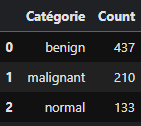
\includegraphics[width=0.8\textwidth]{class_distribution.png}
    \caption{Répartition des classes dans le dataset}
    \label{fig:class_dist}
\end{figure}

\subsection{Analyse Exploratoire (EDA)}
Les résultats clés de notre analyse :

\subsubsection{Caractéristiques des Images}
\begin{table}[h]
    \centering
    \caption{Statistiques des dimensions d'images}
    \begin{tabular}{lcc}
        \toprule
        & Hauteur (px) & Largeur (px) \\
        \midrule
        Minimum & 310 & 190 \\
        Maximum & 719 & 1048 \\
        \bottomrule
    \end{tabular}
    \label{tab:dimensions}
\end{table}

\subsubsection{Analyse des Masques}
\begin{table}[h]
    \centering
    \caption{Superficie tumorale moyenne (en pixels)}
    \begin{tabular}{lcccc}
        \toprule
        Classe & Moyenne & Médiane & Min & Max \\
        \midrule
        Bénin & 20,734 & 10,263 & 804 & 209,121 \\
        Malin & 43,376 & 34,433 & 569 & 167,411 \\
        Normal & 0 & 0 & 0 & 0 \\
        \bottomrule
    \end{tabular}
    \label{tab:masks}
\end{table}

\begin{figure}[h]
    \centering
    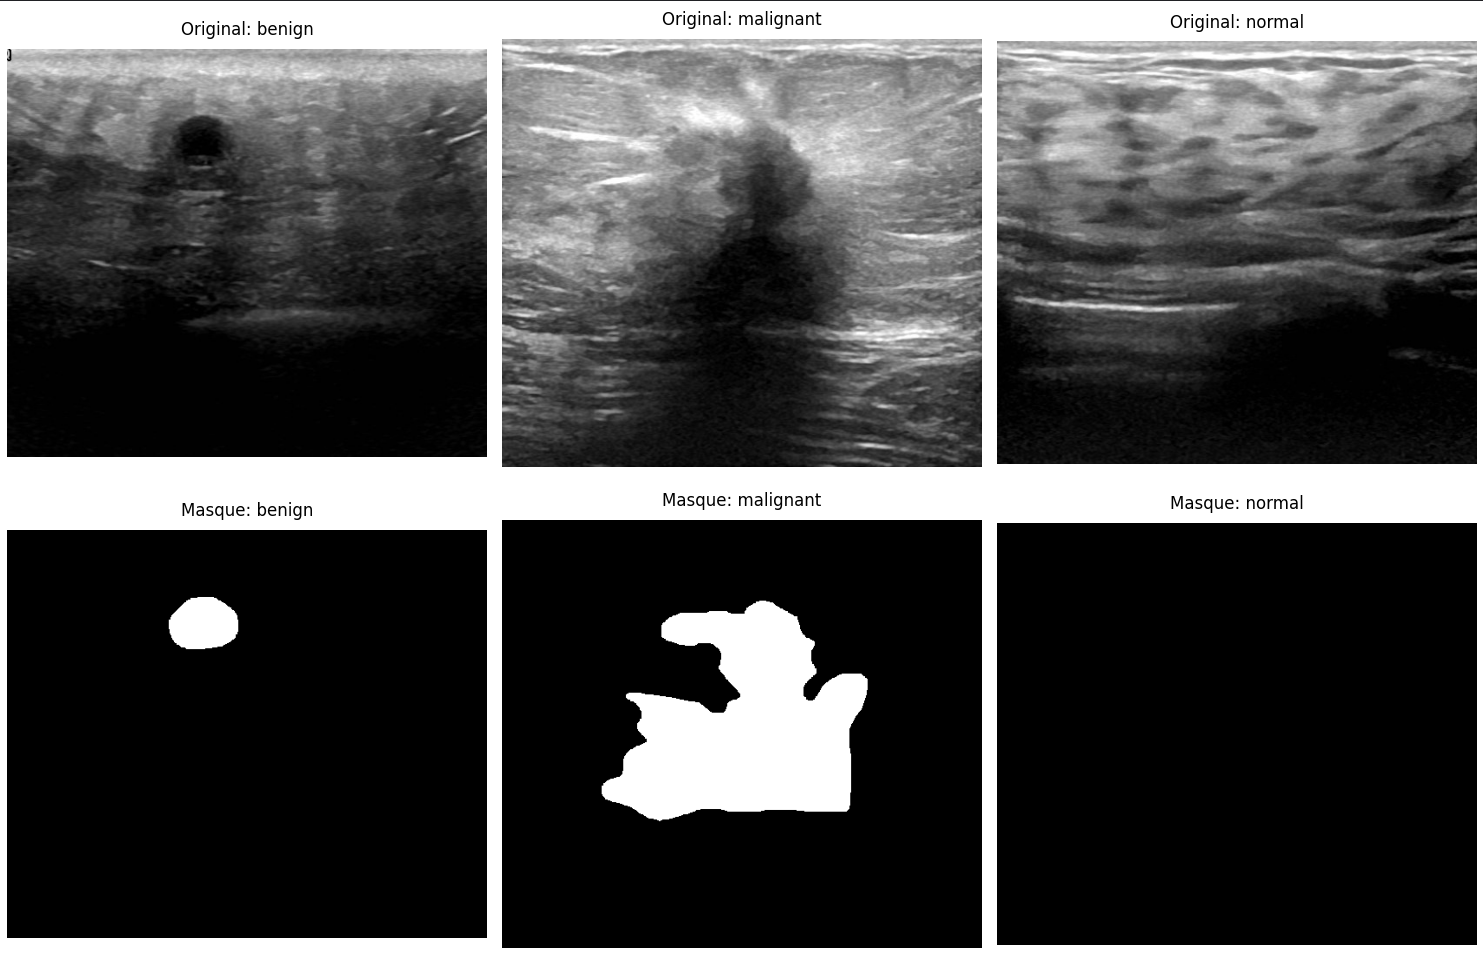
\includegraphics[width=0.8\textwidth]{sample_images.png}
    \caption{Exemples d'images avec leurs masques correspondants}
    \label{fig:samples}
\end{figure}


\section{Adaptations Méthodologiques}
Suite à l'EDA, nous avons ajusté notre approche :

\subsection{Résolution des Problèmes Identifiés}
\begin{itemize}
    \item \textbf{Déséquilibre de classes} : Implémentation d'une fonction de coût pondérée
    \begin{equation}
        w_c = \frac{N}{C \times N_c}
    \end{equation}
    où $N$=total, $C$=classes, $N_c$=échantillons par classe

    \item \textbf{Normalisation des dimensions} : Redimensionnement à $256\times256$ px avec préservation du ratio d'aspect

    \item \textbf{Utilisation des masques} : Intégration comme 4ème canal d'entrée
\end{itemize}

\subsection{Pipeline de Prétraitement}
\begin{enumerate}
    \item Chargement des paires (image, masque)
    \item Redimensionnement avec remplissage intelligent
    \item Augmentation de données :
    \begin{itemize}
        \item Rotation aléatoire ($\pm15^\circ$)
        \item Retournement horizontal
        \item Ajustement de contraste
    \end{itemize}
    \item Normalisation : $\mu=[0.485,0.456,0.406]$, $\sigma=[0.229,0.224,0.225]$
\end{enumerate}

\section{Prochaines Étapes}
\begin{itemize}
    \item Implémentation des architectures CNN (ResNet18, EfficientNet)
    \item Expérimentation avec des mécanismes d'attention
    \item Évaluation comparative des modèles
    \item Optimisation des hyperparamètres
\end{itemize}

\section*{Annexe}
\subsection*{Exemple de Code}
\begin{verbatim}
# Chargement des données
dataset = BreastUltrasoundDataset(
    image_paths=X_train,
    mask_paths=mask_train,
    labels=y_train,
    transform=train_transform
)
\end{verbatim}

\bibliographystyle{plain}
\bibliography{references}

\end{document}